% Paper 3 — Results Section
% Building Local-Language Economic Narrative Indices

\section{Results}\label{sec:results}

\paragraph{Scope of reported results.}
The results in this section combine the legacy Potrika calibration diagnostics with the frozen BENI v1 validation results. The legacy calibration subsections are retained as prototype evidence. The current frozen BENI v1 comparison uses the repaired article-level predictions, the 186-row clean validation subset, and the regenerated monthly index files.

\subsection{Model Comparison}

Table~\ref{tab:model-comparison} reports per-model performance on the frozen BENI v1 validation set (186 articles, 69 Economic, 117 Not Economic). The repaired TF-IDF model achieves 88.17\% accuracy and 0.823 F1 on the Economic class. The majority-class baseline is included only as a sanity check and is not competitive on the minority class.

\begin{table}[h]
\centering
\begin{tabular}{lccccc}
\toprule
Model & Acc. & $\kappa$ & Prec. & Rec. & F1 \\
\midrule
TF-IDF + LogReg & 88.17\% & 0.736 & 92.73\% & 73.91\% & 0.823 \\
Majority baseline (Not Economic) & 62.90\% & 0.000 & 0.00\% & 0.00\% & 0.000 \\
\bottomrule
\end{tabular}
\caption{Per-model performance vs. the frozen BENI v1 validation set (n=186). The TF-IDF model is the production baseline for the frozen release. The majority baseline is included as a reference only.}
\label{tab:model-comparison}
\end{table}

The frozen validation result is materially stronger than the majority baseline, but it is still a conservative estimate because 114 ambiguous rows were excluded from clean validation. The TF-IDF model identifies 51 of 69 Economic articles correctly, with only 4 false positives. Legacy BanglaBERT comparison results are retained in the supplementary prototype files, but they are not used in the frozen BENI v1 validation table.

\paragraph{Error overlap.} Of the 33 articles where at least one weak-label model disagrees with the silver standard, 8 articles (24\%) are misclassified by \textit{both} models. These joint errors span genuine borderline cases: political party funding, mobile phone discounts, agricultural loan programs, and energy sector reporting---articles where the economic framing is ambiguous even for the LLM annotator (self-consistency $\kappa = 0.48$ on these types). This pattern is consistent with a shared weak-label ceiling rather than model-specific weaknesses.

\subsection{Active Learning Curve}

Figure~\ref{fig:active-learning} shows the active learning simulation results using TF-IDF + Logistic Regression with 5-fold stratified cross-validation (25 trials per budget).

\begin{figure}[h]
\centering
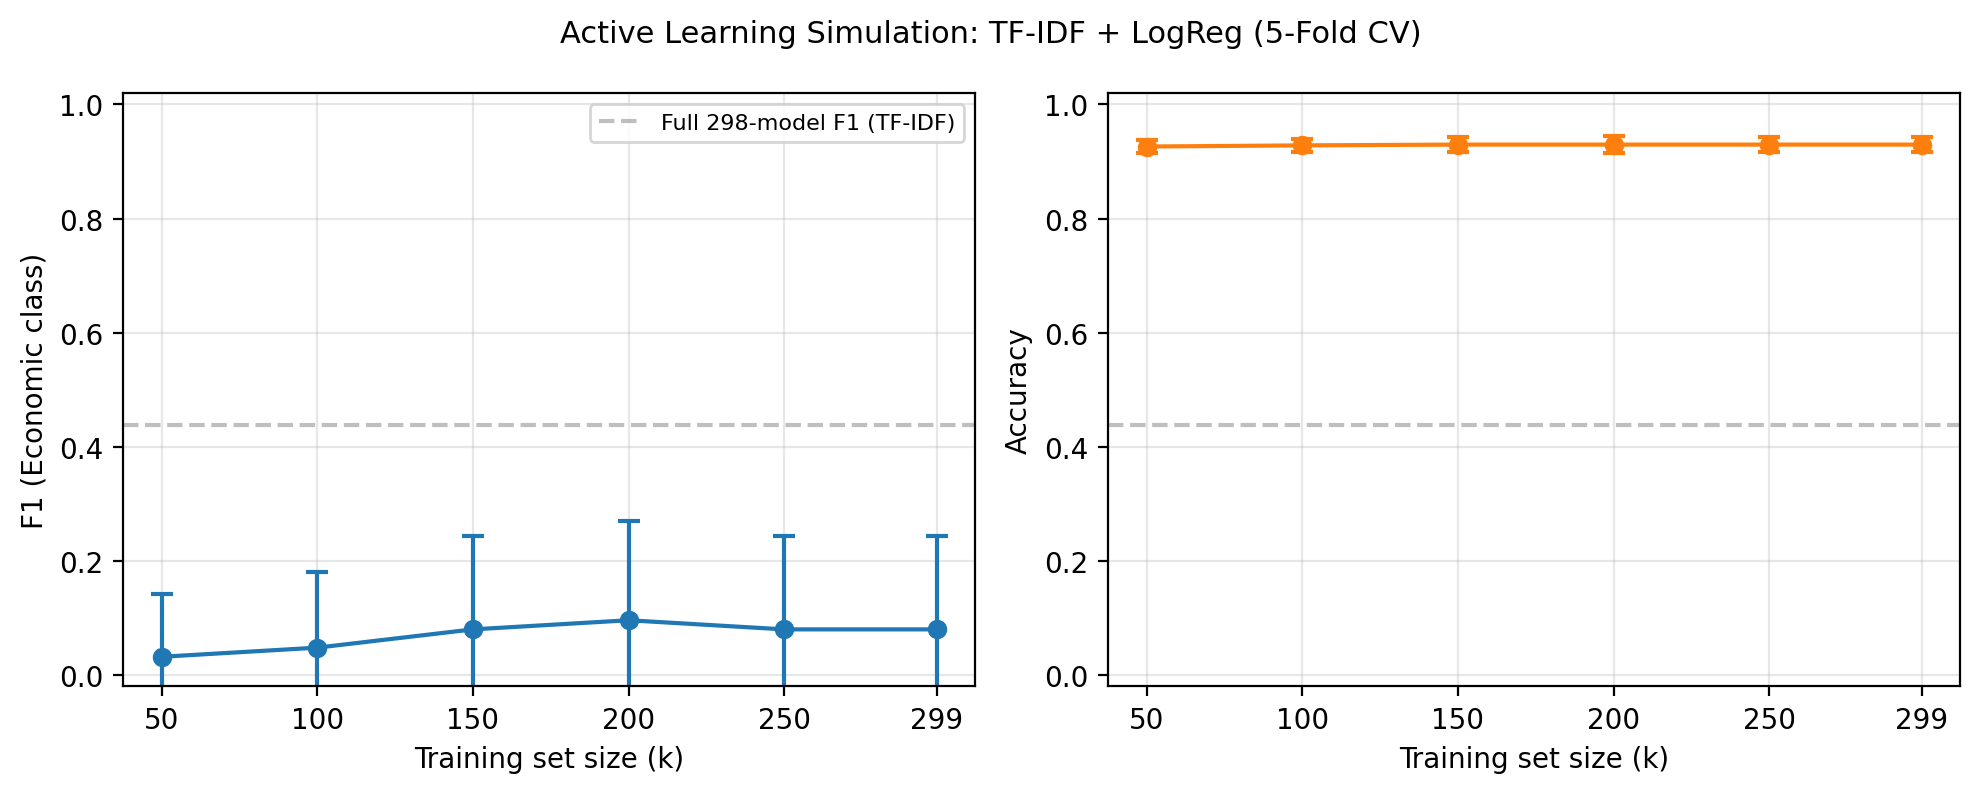
\includegraphics[width=\textwidth]{../../data/annotations/active_learning_plot.png}
\caption{Legacy active learning simulation: F1 (Economic class) and accuracy vs. annotation budget $k$. Error bars show $\pm1$ standard deviation across 25 trials. The gray dashed line marks the full-data TF-IDF F1 of 0.44. Accuracy hovers at $\sim$93\% at every budget---the majority-class baseline---while F1 never exceeds 0.10.}
\label{fig:active-learning}
\end{figure}

The curve is flat. At every budget from $k = 50$ to $k = 299$, accuracy remains at the majority-class baseline ($\sim$93\%), and F1 for the Economic class never exceeds 0.10. The classifier defaults to ``Not Economic'' for the vast majority of test articles at every budget, reflecting the fundamental difficulty of learning a minority class from 3--18 positive training examples at a 7.4\% base rate.

This result is informative as a \textit{lower bound}: with 299 articles and 22 positives, even TF-IDF---our best weak-label model---cannot overcome the base-rate problem. The minimum viable annotation budget for rare-event economic text classification with linear classifiers is substantially larger than $k = 300$, or requires a stronger model (e.g., the LLM annotator itself) or a designed sampling strategy (e.g., uncertainty sampling or positive-unlabeled learning).

\subsection{Correlation with Macroeconomic Indicators}

Table~\ref{tab:correlations} reports the relationship between the prototype monthly BENI calibration index and two key macroeconomic indicators for Bangladesh: the BDT/USD exchange rate and the CPI.

\begin{table}[h]
\centering
\begin{tabular}{lcccc}
\toprule
 & \multicolumn{2}{c}{Level} & \multicolumn{2}{c}{First-differenced} \\
\cmidrule(lr){2-3} \cmidrule(lr){4-5}
Indicator & $r$ & $p$ & $r$ & $p$ \\
\midrule
BDT/USD exchange rate & $-$0.72 & $<$0.001 & 0.10 & 0.38 \\
CPI (all items) & $-$0.75 & $<$0.001 & $-$0.04 & 0.73 \\
\bottomrule
\end{tabular}
\caption{Pearson correlations between the prototype monthly BENI calibration index and macroeconomic indicators. Level correlations are strong and negative; first-differenced correlations are negligible and statistically insignificant.}
\label{tab:correlations}
\end{table}

The level correlations ($-$0.72 with FX, $-$0.75 with CPI) indicate long-run co-movement in the calibration window: the prototype economic-news share declines over 2014--2020 while the exchange rate and consumer-price index trend upward. This pattern is useful for measurement validation, but it should not be interpreted as causal evidence or as out-of-sample forecasting performance.

The first-differenced correlations, however, are statistically indistinguishable from zero ($r = 0.10$, $p = 0.38$ for FX; $r = -0.04$, $p = 0.73$ for CPI). This means month-to-month changes in the prototype economic-news share do not predict month-to-month changes in exchange rates or consumer prices. We interpret this null result as evidence that economic narrative salience may be a long-run measurement signal rather than a short-run forecasting signal. Section~\ref{sec:discussion} examines this distinction in detail.

\paragraph{Lead correlations.} Leading BENI by 1, 3, and 6 months against the macro indicators produces similar level correlations ($r$ between $-$0.72 and $-$0.74, all $p < 0.001$), reflecting the same trend co-movement rather than predictive lead-lag relationships.
